\documentclass[landscape]{beamer}
\usepackage{xcolor}
\usepackage{amsmath, amsthm}
\newtheorem{benchmark}{Benchmark}
\newtheorem{environment}{Environment}
\newtheorem{distribution}{The Distribution of Counting Operators in Our Benchmark}
\usepackage{mathrsfs}
\usepackage{hyperref}
\usepackage{algpseudocode}
\usepackage{tikz}
\usetikzlibrary {decorations.pathmorphing, curvilinear, shadows,shapes.symbols, automata, positioning, shapes,arrows, matrix}
\usepackage{multicol}
\usepackage{pgfplots}
\usepackage{array}
\usepackage{colortbl}
\definecolor{grayshade}{gray}{0.9}
\usepackage{listings}
\lstdefinestyle{myjs}{
  language=C,
  basicstyle=\ttfamily,
  keywordstyle=\color{blue},
  stringstyle=\color{red},
  commentstyle=\color{green},
  backgroundcolor=\color{gray!10},
  breaklines=true,
  frame=single,
  captionpos=b
}
\usepackage{booktabs}
\usepackage{siunitx}

\linespread{1.5}
\newcommand{\aut}{\mathcal{A}}
\newcommand{\myvec}[1]{\overrightarrow{#1}}
\newcommand{\cB}{\mathcal{B}}
\newcommand{\anivar}{\mathfrak{x}}
\newcommand*{\ostrichrecl}{\rm OSTRICH^{RECL}}

\colorlet{noteColor}{green!10!orange}

\mode<presentation> {

\usetheme{Singapore}


\useinnertheme{rounded}

\useoutertheme{split}

\usefonttheme{professionalfonts}
}


%------------------------------------------------------------
%This block of code defines the information to appear in the
%Title page
\graphicspath{{pics/}}

\title{String Constraints with Regex-Counting and
String-Length Solved More Efficiently}
\author{\textbf{Denghang Hu}, Zhilin Wu}
\institute{Institute of Software, University of Chinese Academy of Sciences}

% Add the image inside titlegraphics macro
\titlegraphic{
  
\includegraphics[width=0.2\textwidth]{pics/ISCAS-logo.jpeg} \quad\quad\quad\quad
  
\includegraphics[width=0.3\textwidth]{pics/ucas_logo.pdf}
}

%End of title page configuration block
%------------------------------------------------------------

%------------------------------------------------------------
%The next block of commands puts the table of contents at the 
%beginning of each section and highlights the current section:

\AtBeginSection[]
{
  \begin{frame}
    \tableofcontents[currentsection]
  \end{frame}
}
%------------------------------------------------------------

\begin{document}

\pdfbookmark{Title}{Title}
%The next statement creates the title page.
\frame{\titlepage}

% no more than 15 mins 
% Introduction : (3min)
% 1 Motivation
% 3 contribution of our work (overview)
\section{Introduction}

\begin{frame}{String is Important}
  \textbf{String is a primitive data type in program languages:}
  \begin{itemize}
    \item C/++/\#
    \item Java
    \item JavaScript/TypeScript
    \item Python
    \item Go
    \item ...
  \end{itemize}
\end{frame}

\begin{frame}{String is Widely Used in Security-Critical Situations}
  \begin{itemize}
    \item Input sanitisation, validation
    \item Quary generation for databases
    \item Data handling: XML, JSON, HTML
    \item Dynamic code generation
    \item ...
  \end{itemize}
\end{frame}


\begin{frame}
  \frametitle{String is Error-Prone}
  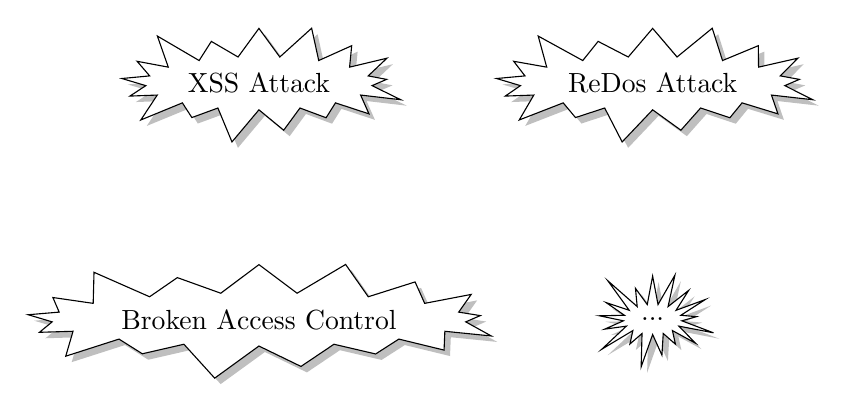
\begin{tikzpicture}
    \node[starburst,drop shadow,fill=white,draw] at (0,0) {XSS Attack};
    \node[starburst,drop shadow,fill=white,draw] at (5,0) {ReDos Attack};
    \node[starburst,drop shadow,fill=white,draw] at (0,-3) {Broken Access Control};
    \node[starburst,drop shadow,fill=white,draw] at (5,-3) {...};
  \end{tikzpicture}
\end{frame}

\begin{frame}[fragile]{Detect Attacks by String Constraints}
  \textbf{Malicious User Input:}
  \begin{lstlisting}[style=myjs]
      <script> XSSAtack </script>
    \end{lstlisting}
  \textbf{Security String Constraints:}
  \begin{lstlisting}[style=myjs]
    (assert (not (str.contains x '<script>')))
  \end{lstlisting}
\end{frame}

\begin{frame}
  \frametitle{String Solvers}
  \begin{multicols}{2}
    \begin{itemize}
      \item ABC
      \item CVC3/4/5
      \item Gecode+S
      \item OSTRICH
      \item Stranger
      \item S3/p/\#
      \item Sloth
      \item SLENT
      \item TRAU/+
      \item Woorpje
      \item Z3str2/3/4/RE/Seq
      \item ...
    \end{itemize}
  \end{multicols}
\end{frame}


\begin{frame}{But...}
  \textbf{Existing Solvers Cannot Solve:}
  \begin{tikzpicture}
    \node (formula) at (0,0) {
      $
        x\in (\Sigma / a)^{\{1,60\}}(\Sigma / b)^{\{1,60\}}(\Sigma / c)^{\{0,60\}} \wedge x\in \Sigma^*c^+ \wedge |x| > 120
      $
    };
    \node [rotate=45, scale=2, text=red!60, fill=yellow!20,draw,decorate,decoration={bumps,mirror}, opacity=0] at (1,0) {300s TIMEOUT};
  \end{tikzpicture}
\end{frame}
\begin{frame}{But...}
  \textbf{Existing Solvers Cannot Solve:}
  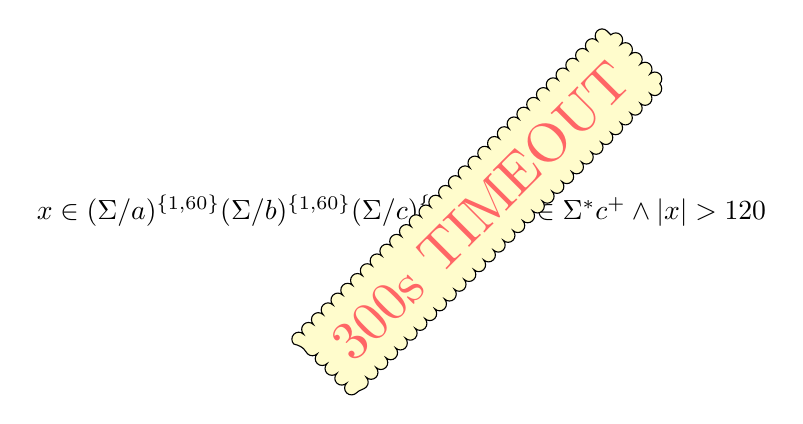
\begin{tikzpicture}
    \node (formula) at (0,0) {
      $
        x\in (\Sigma / a)^{\{1,60\}}(\Sigma / b)^{\{1,60\}}(\Sigma / c)^{\{0,60\}} \wedge x\in \Sigma^*c^+ \wedge |x| > 120
      $
    };
    \node [rotate=45, scale=2, text=red!60, fill=yellow!20,draw,decorate,decoration={bumps,mirror}] at (1,0) {300s TIMEOUT};
  \end{tikzpicture}
\end{frame}


\begin{frame}[fragile]
  \frametitle{However ...}
  \textbf{Regex-Countings are Widely Used}
  \begin{table}
    \centering
    \begin{tabular}{l l l S[table-format=1.2]}
      \toprule
      \textbf{Rank} & \textbf{Type}  & \textbf{Example} & \textbf{\% Projects} \\
      \midrule
      1             & $\cdot\{1,\}$  & $z^+$            & 0.1                  \\
      3             & $\cdot\{0,\}$  & $z^*$            & 0.2                  \\
      18            & $\cdot\{n\}$   & $z\{8\}$         & 0.05                 \\
      20            & $\cdot\{n,m\}$ & $z\{8,9\}$       & 0.3                  \\
      \bottomrule
    \end{tabular}
    \caption{The Rank and Percentage of Regex-Countings in Python \footnote{Chapman,C. et al: Exploring regular expression usage and context in python}}
  \end{table}

\end{frame}

\begin{frame}[fragile]
  \frametitle{However ...}
  \textbf{String-Length is Widely Used}
  \begin{figure}
    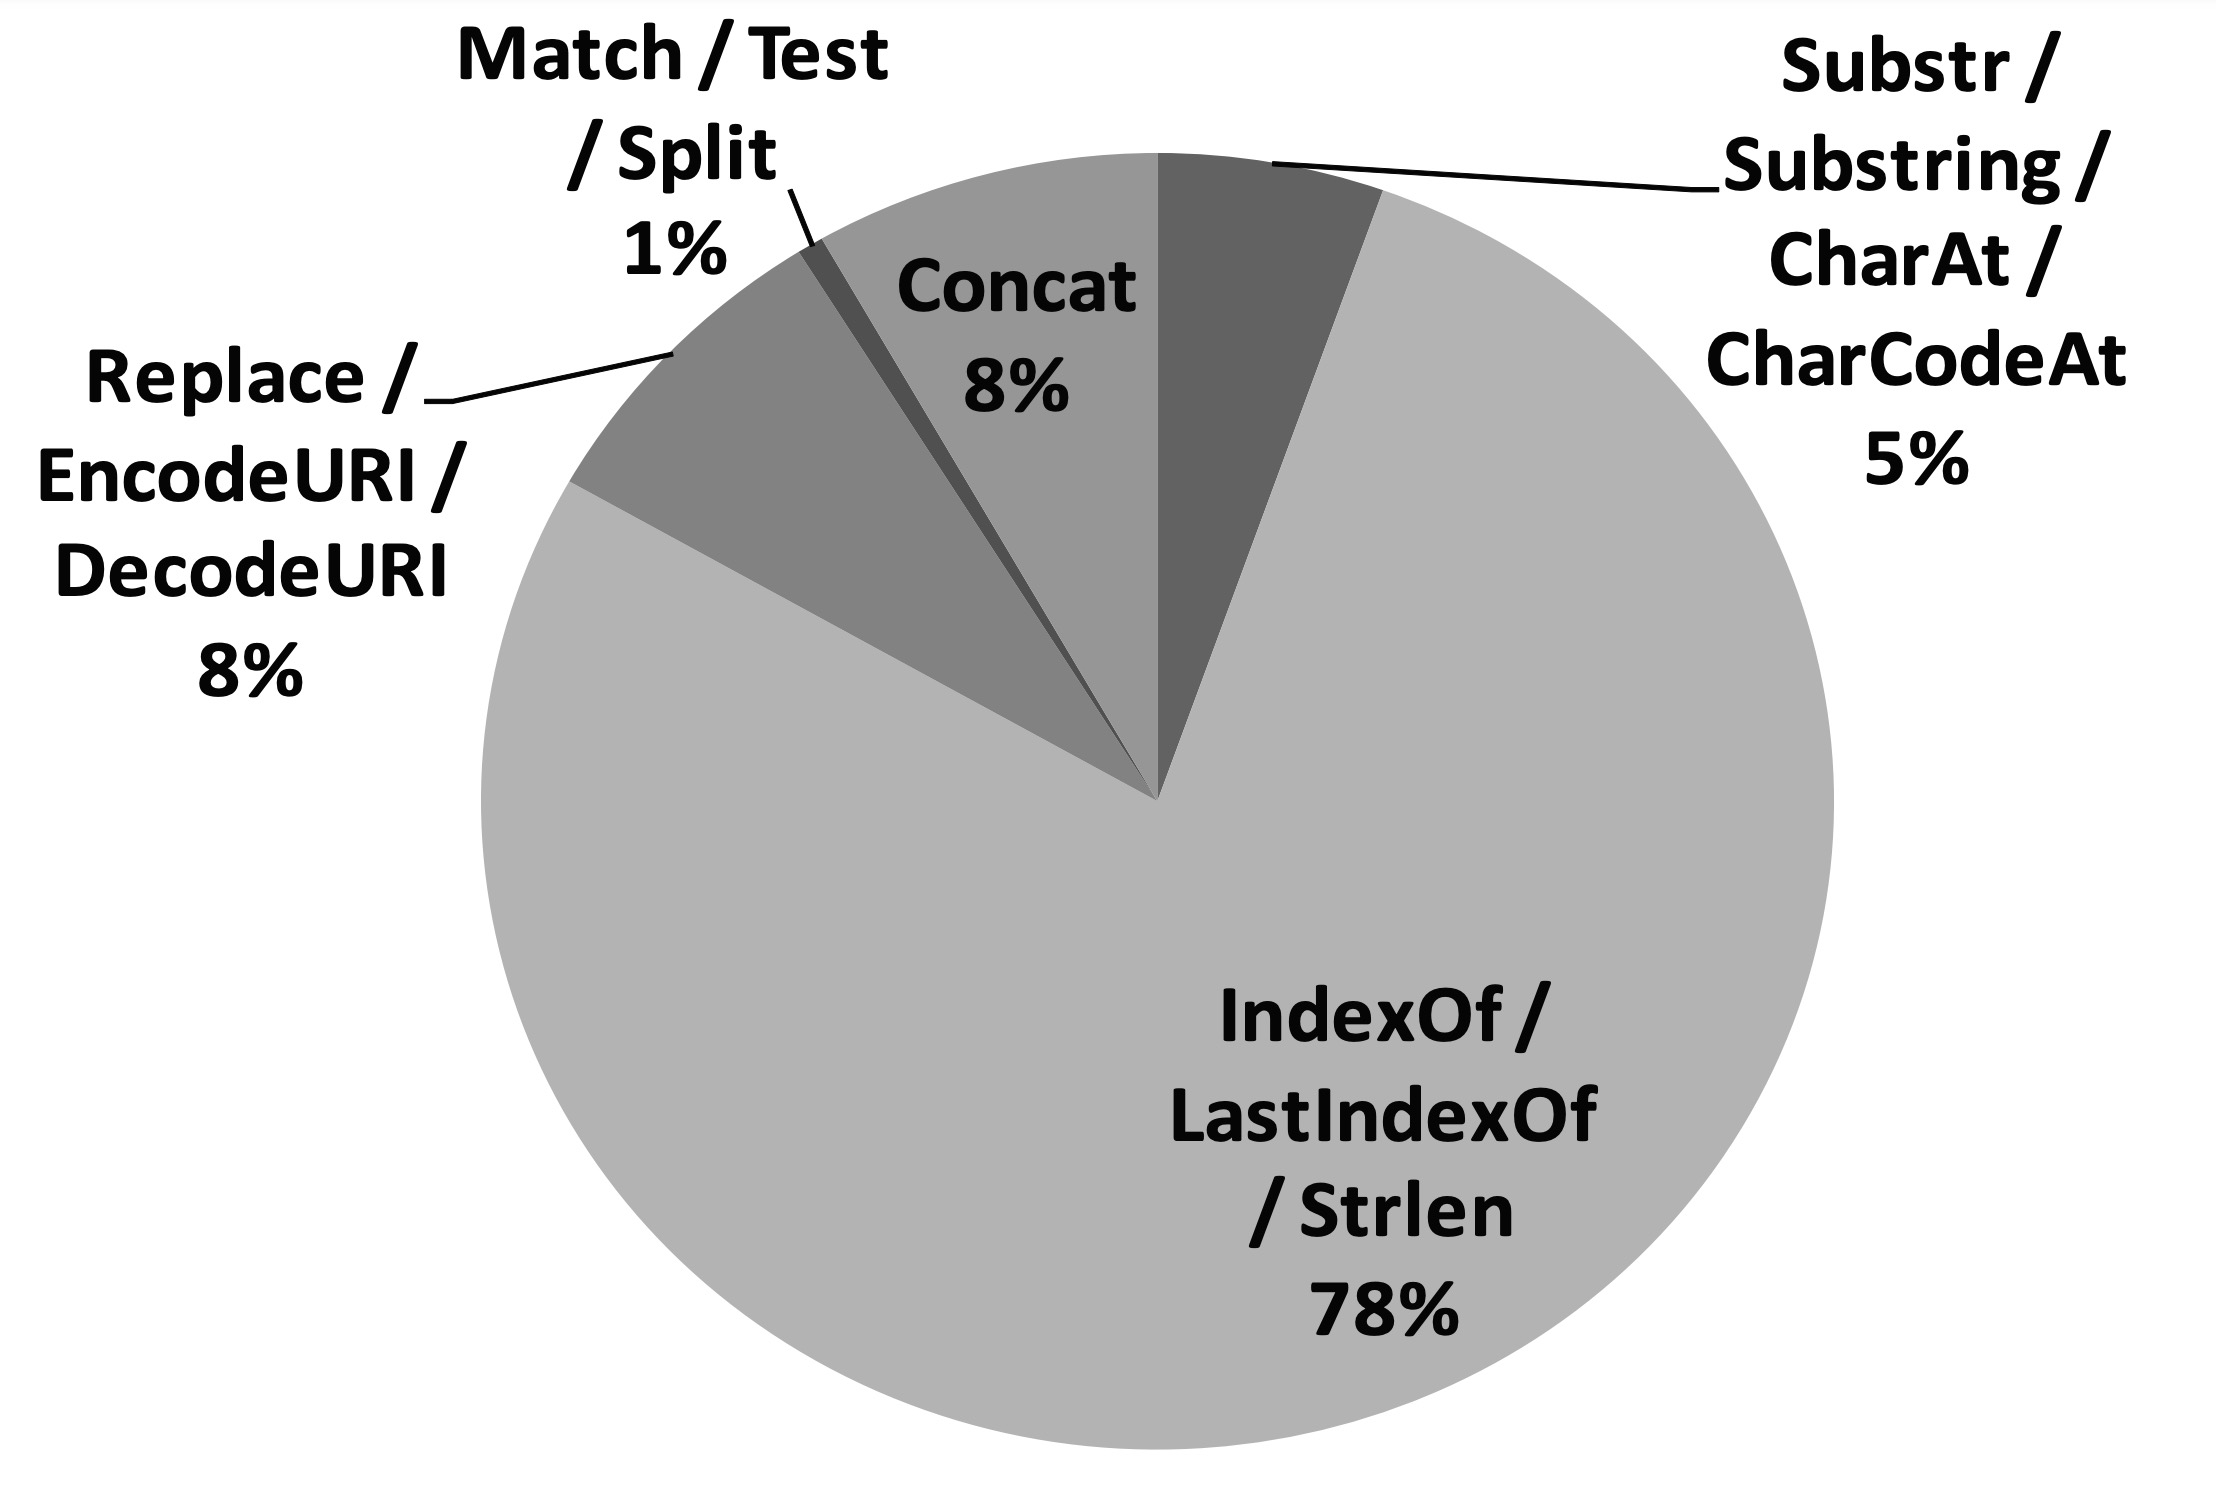
\includegraphics[width=.5\linewidth]{length_percentage.jpg}
    \caption{The Percentages of String Operations in Web Applications \footnote{Saxena, P. et al: A symbolic execution framework for JavaScript.}}
  \end{figure}
\end{frame}

% Technical details : (8min)
% 1 What is Regex-Counting
% 2 normal ways (z3, cvc5, trau)
% 3 our ways
%   1 An example (5-7 pages)
%   2 Decisino procedure 1 pages
\section{Our Approach}
\begin{frame}{Example}
  \begin{tikzpicture}
    \node (placeholder) at (0,0) {
      $
        x\in (\Sigma / a)^{\{1,60\}}(\Sigma / b)^{\{1,60\}}(\Sigma / c)^{\{0,60\}} \wedge x\in \Sigma^*c^+ \wedge |x| > 120
      $
    };
    \node [rotate=45, scale=2, text=red!60, fill=yellow!20,draw,decorate,decoration={bumps,mirror}, opacity=0] at (1,0) {300s TIMEOUT};
  \end{tikzpicture}
\end{frame}

\begin{frame}{Exsiting Techniques to Such Constraints}
  \begin{tikzpicture}
    \node [anchor=north, anchor=west, align=left, text width = \linewidth] (text) at (-3,0) {
      Rule-based (CVC5, Z3): \textbf{Repeatly unroll} counting operators by derivation rules. For example,
      $x\in \Sigma\cdot z \wedge z\in \Sigma^*c^+$ is derived from $x\in \Sigma^*c^+$ in CVC5.
    };
    \node (cvc5) at (0,-3) {
      
\includegraphics[width=0.4\linewidth]{cvc5_logo.png}
    };
    \node (z3) at (5,-3) {
      
\includegraphics[width=0.2\linewidth]{Z3_logo.jpeg}
    };
    \node [align=left,rotate=45, scale=2, text=red!60, fill=yellow!20,draw,decorate,decoration={bumps,mirror},opacity=0] at (5,-3) {Exponentially Search ?};
  \end{tikzpicture}
\end{frame}
\begin{frame}{Exsiting Techniques to Such Constraints}
  \begin{tikzpicture}
    \node [anchor=north, anchor=west, align=left, text width = \linewidth] (text) at (-3,0) {
      Rule-based (CVC5, Z3): \textbf{Repeatly unroll} counting operators by derivation rules. For example,
      $x\in \Sigma\cdot z \wedge z\in \Sigma^*c^+$ is derived from $x\in \Sigma^*c^+$ in CVC5.
    };
    \node (cvc5) at (0,-3) {
      
\includegraphics[width=0.4\linewidth]{cvc5_logo.png}
    };
    \node (z3) at (5,-3) {
      
\includegraphics[width=0.2\linewidth]{Z3_logo.jpeg}
    };
    \node [align=left,rotate=45, scale=2, text=red!60, fill=yellow!20,draw,decorate,decoration={bumps,mirror}] at (5,-3) {\uppercase{Exponential ?}};
  \end{tikzpicture}
\end{frame}


\begin{frame}{Exsiting Techniques to Such Constraints}
  \begin{tikzpicture}
    \node [anchor=north, anchor=west, align=left, text width = \linewidth] (text) at (-3,0) {
      Automaton-based (Z3Str3RE, OSTRICH):\textbf{ Syntactically unwind} counting operators and then construct automata. E.g., $(\Sigma/a)^{\{1,60\}}$ is unwound to $\Sigma/a\mid \Sigma/a \Sigma/a \mid \cdots$
    };
    \node (z3) at (0,-3) {
      
\includegraphics[width=0.2\linewidth]{Z3_logo.jpeg}
    };
    \node (ostrich) at (5,-3) {
      
\includegraphics[width=0.3\linewidth]{ostrich_logo.jpeg}
    };
    \node [rotate=45, scale=2, text=red!60, fill=yellow!20,draw,decorate,decoration={bumps,mirror},opacity=0] at (5,-3) {STATE EXPLOSION ?};
  \end{tikzpicture}
\end{frame}
\begin{frame}{Exsiting Techniques to Such Constraints}
  \begin{tikzpicture}
    \node [anchor=north, anchor=west, align=left, text width = \linewidth] (text) at (-3,0) {
      Automaton-based (Z3Str3RE, OSTRICH):\textbf{ Syntactically unwind} counting operators and then construct automata. E.g., $(\Sigma/a)^{\{1,60\}}$ is unwound to $\Sigma/a\mid \Sigma/a \Sigma/a \mid \cdots$
    };
    \node (z3) at (0,-3) {
      
\includegraphics[width=0.2\linewidth]{Z3_logo.jpeg}
    };
    \node (ostrich) at (5,-3) {
      
\includegraphics[width=0.3\linewidth]{ostrich_logo.jpeg}
    };
    \node [rotate=45, scale=2, text=red!60, fill=yellow!20,draw,decorate,decoration={bumps,mirror}] at (5,-3) {STATE EXPLOSION ?};
  \end{tikzpicture}
\end{frame}

\begin{frame}{Our Techniques to Such Constraints}
  \begin{itemize}
    \item Automata with integer registers
    \item Encode counting operators by registers (no explicitly unwind)
    \item Size reduction techniques for automata
  \end{itemize}
\end{frame}

\begin{frame}{Intuition}
  \begin{tikzpicture}[anchor=west]
    \node (a_1_3) at (0, 0) {
      \begin{tikzpicture}[node distance=0.5cm, auto,semithick, font =\small, initial text=$a^{\{1,3\}}:$,
          every state/.style={inner sep=1pt, minimum size=5pt}]
        \node[state,initial] (q0) {$q_0$};
        \node[state, accepting] (q1) [right=of q0] {$q_1$};
        \node[state, accepting] (q2) [right=of q1] {$q_2$};
        \node[state, accepting] (q3) [right=of q2] {$q_3$};
        \path[->]
        (q0) edge [above] node {$a$} (q1)
        (q1) edge [above] node {$a$} (q2)
        (q2) edge [above] node {$a$} (q3);
      \end{tikzpicture}
    };
    \node (text1) at (6,0) {\textbf{Finite Automata}};
    \node [opacity = 0] (a_star) at (0,-2) {
      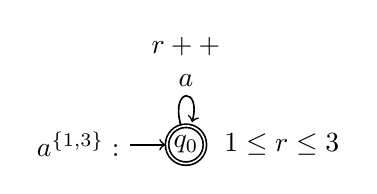
\begin{tikzpicture}[node distance=0.1cm, auto,semithick,  initial text=$a^{\{1,3\}}:$,
          every state/.style={inner sep=1pt, minimum size=5pt}]
        \node[state,initial,accepting] (q0) {$q_0$};
        \node (accepting_condition) [right=of q0] {$1\leq r\leq3$};
        \path[->]
        (q0) edge [loop above] node [align=center] {$r++$ \\ $a$} (q0);
      \end{tikzpicture}
    };
    \node [opacity = 0] (text2) at (6,-2) {\textbf{Extended with Registers}};
  \end{tikzpicture}
\end{frame}
\begin{frame}[fragile]{Intuition}
  \begin{tikzpicture}[anchor=west]
    \node (a_1_3) at (0, 0) {
      \begin{tikzpicture}[node distance=0.5cm, auto,semithick, initial text=$a^{\{1,3\}}:$,
          every state/.style={inner sep=1pt, minimum size=5pt}]
        \node[state,initial] (q0) {$q_0$};
        \node[state, accepting] (q1) [right=of q0] {$q_1$};
        \node[state, accepting] (q2) [right=of q1] {$q_2$};
        \node[state, accepting] (q3) [right=of q2] {$q_3$};
        \path[->]
        (q0) edge [above] node {$a$} (q1)
        (q1) edge [above] node {$a$} (q2)
        (q2) edge [above] node {$a$} (q3);
      \end{tikzpicture}
    };
    \node (text1) at (6,0) {\textbf{Finite Automata}};
    \node (a_star) at (0,-2) {
      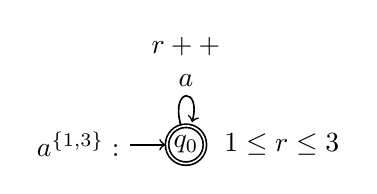
\begin{tikzpicture}[node distance=0.1cm, auto,semithick,  initial text=$a^{\{1,3\}}:$,
          every state/.style={inner sep=1pt, minimum size=5pt}]
        \node[state,initial,accepting] (q0) {$q_0$};
        \node (accepting_condition) [right=of q0] {$1\leq r\leq3$};
        \path[->]
        (q0) edge [loop above] node [align=center] {$r++$ \\ $a$} (q0);
      \end{tikzpicture}
    };
    \node [align=center] (text2) at (6,-2.5) {\textbf{Extended with Registers}\\\textbf{(CEFA)}};

  \end{tikzpicture}
\end{frame}

\begin{frame}{$ x\in \textcolor{red}{(\Sigma / a)^{\{1,60\}}(\Sigma / b)^{\{1,60\}}(\Sigma / c)^{\{0,60\}}} \wedge x\in \Sigma^*c^+ \wedge |x| > 120$}
  \textbf{1. Encode Counting Operators : }
  \begin{figure}
    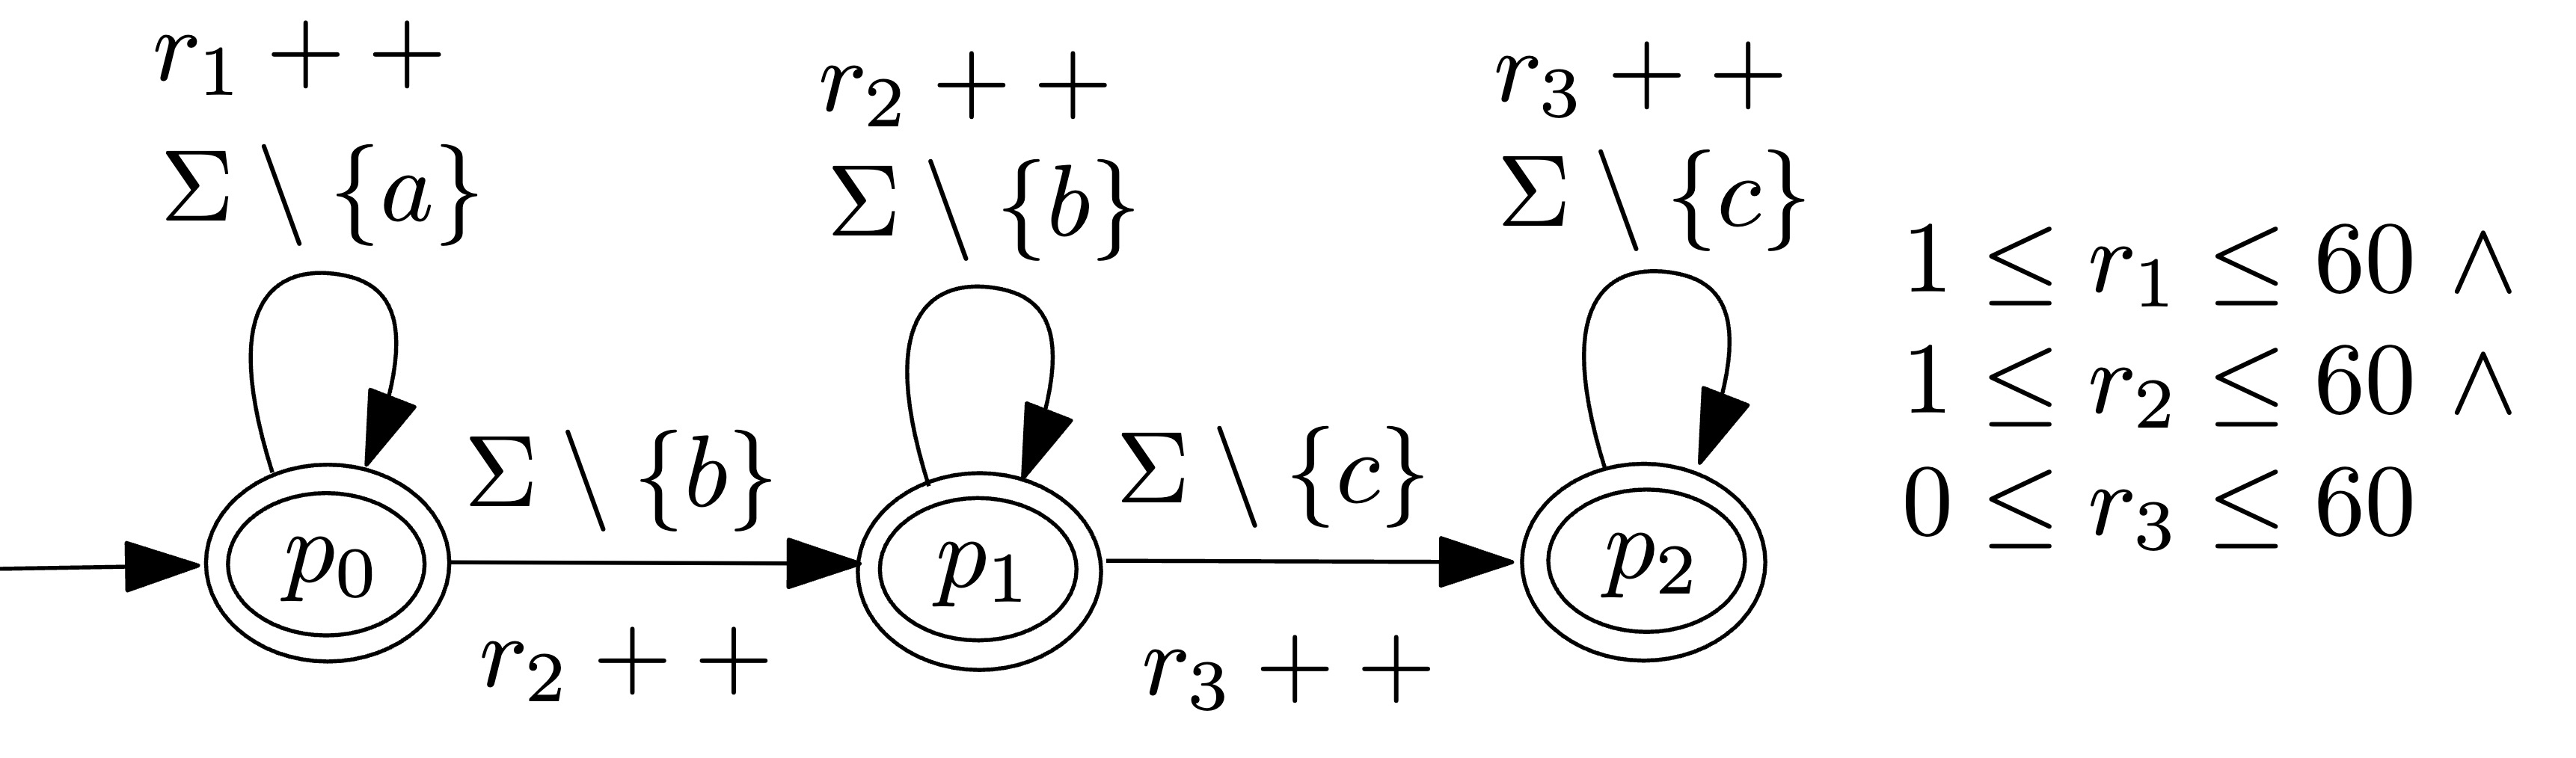
\includegraphics[width=\linewidth]{overview_regex1.jpg}
  \end{figure}
\end{frame}
\begin{frame}{$ x\in (\Sigma / a)^{\{1,60\}}(\Sigma / b)^{\{1,60\}}(\Sigma / c)^{\{0,60\}} \wedge x\in \textcolor{red}{\Sigma^*c^+} \wedge |x| > 120$}
  \textbf{1. Basic Regex Operations : }
  \begin{figure}
    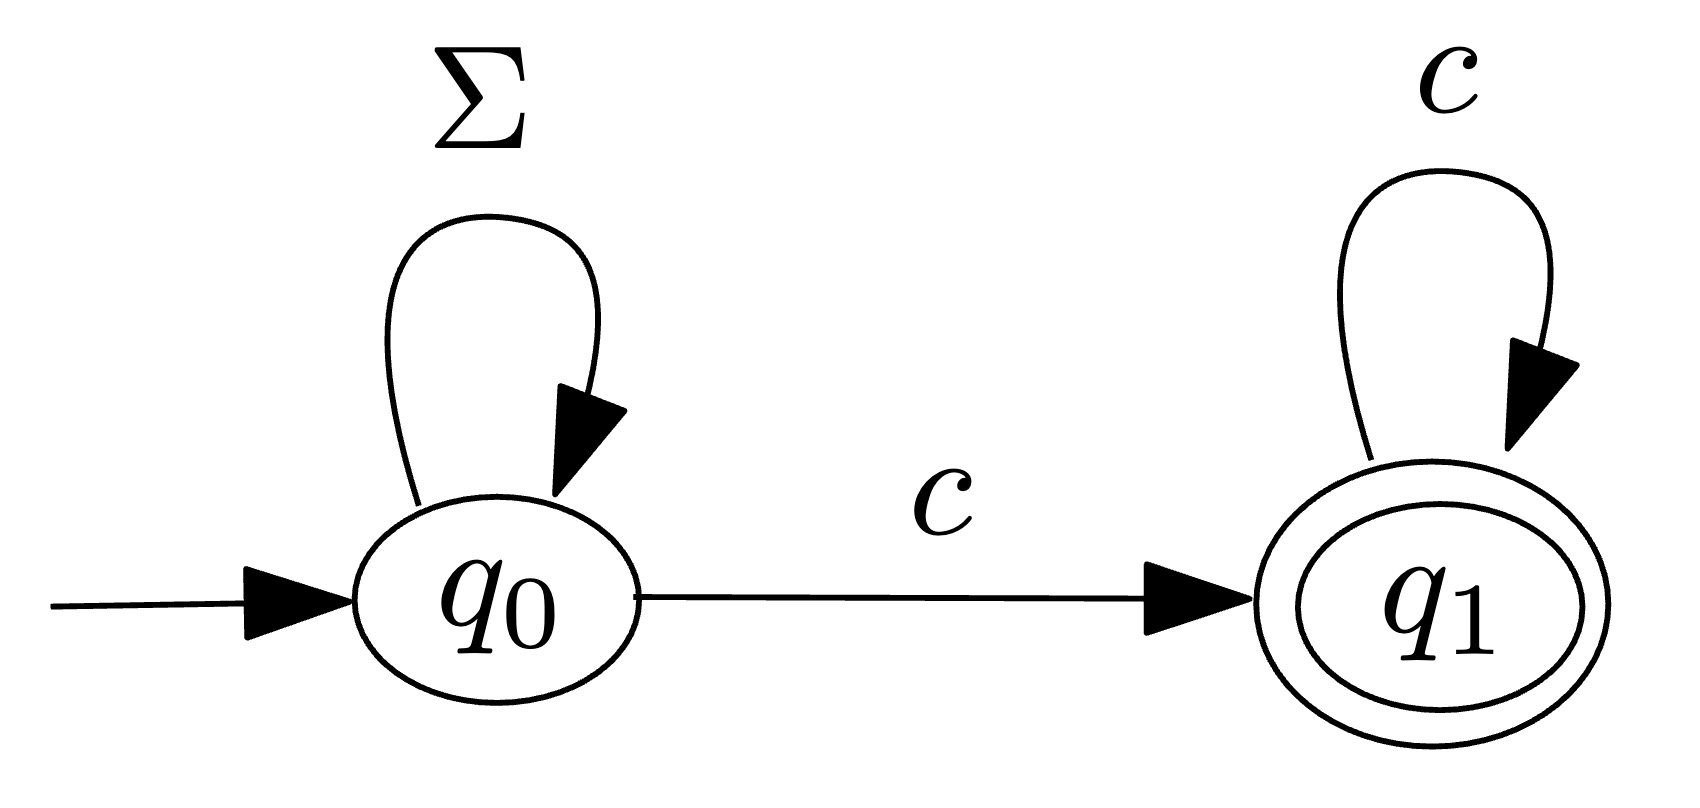
\includegraphics[width=.5\linewidth]{overview_regex2.jpg}
  \end{figure}
\end{frame}
\begin{frame}{$ x\in (\Sigma / a)^{\{1,60\}}(\Sigma / b)^{\{1,60\}}(\Sigma / c)^{\{0,60\}} \wedge x\in \Sigma^*c^+ \wedge \textcolor{red}{|x|} > 120$}
  \textbf{1. The Pre-Image of String-Length :}
  \begin{figure}
    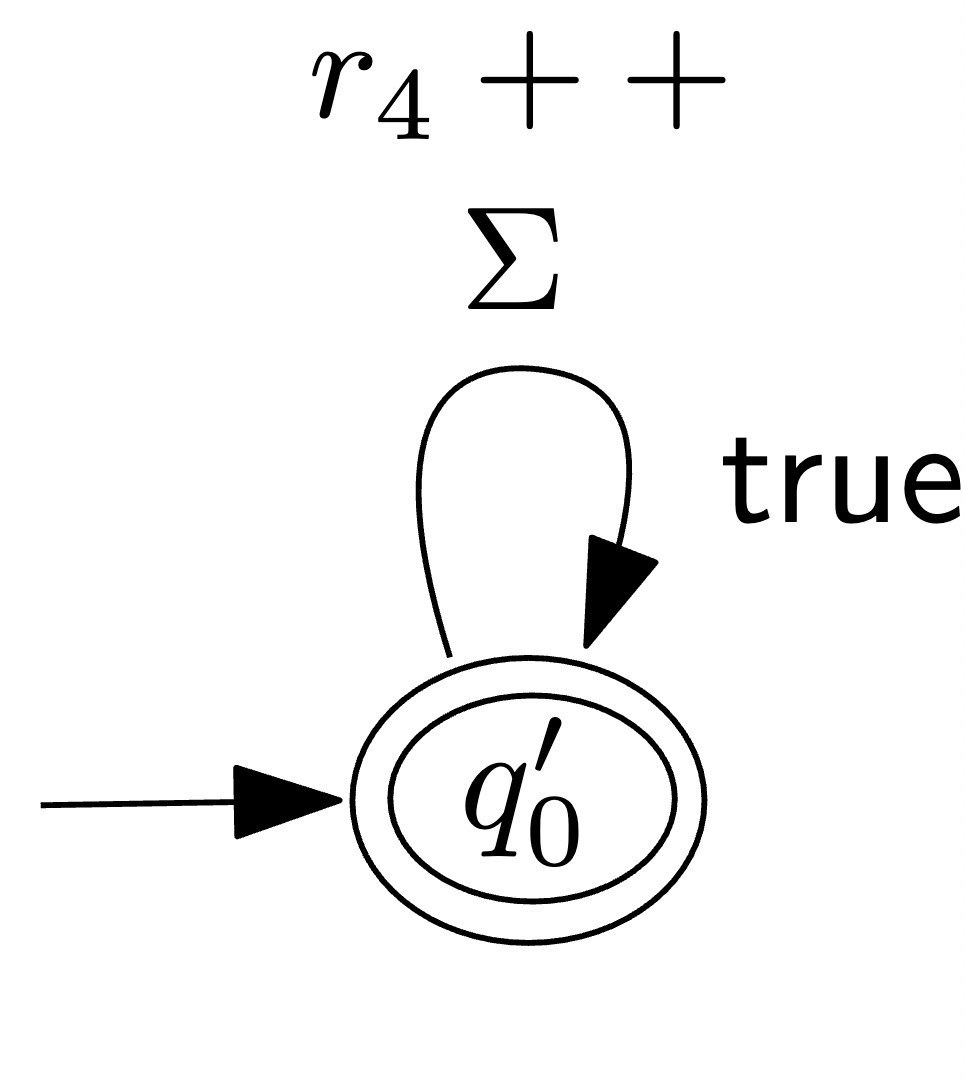
\includegraphics[width=.25\linewidth]{overview_length_pre.jpg}
  \end{figure}
\end{frame}


\begin{frame}{$ x\in (\Sigma / a)^{\{1,60\}}(\Sigma / b)^{\{1,60\}}(\Sigma / c)^{\{0,60\}} \wedge x\in \Sigma^*c^+ \wedge |x| > 120$}
  \textbf{2. Production : }
  \begin{figure}
    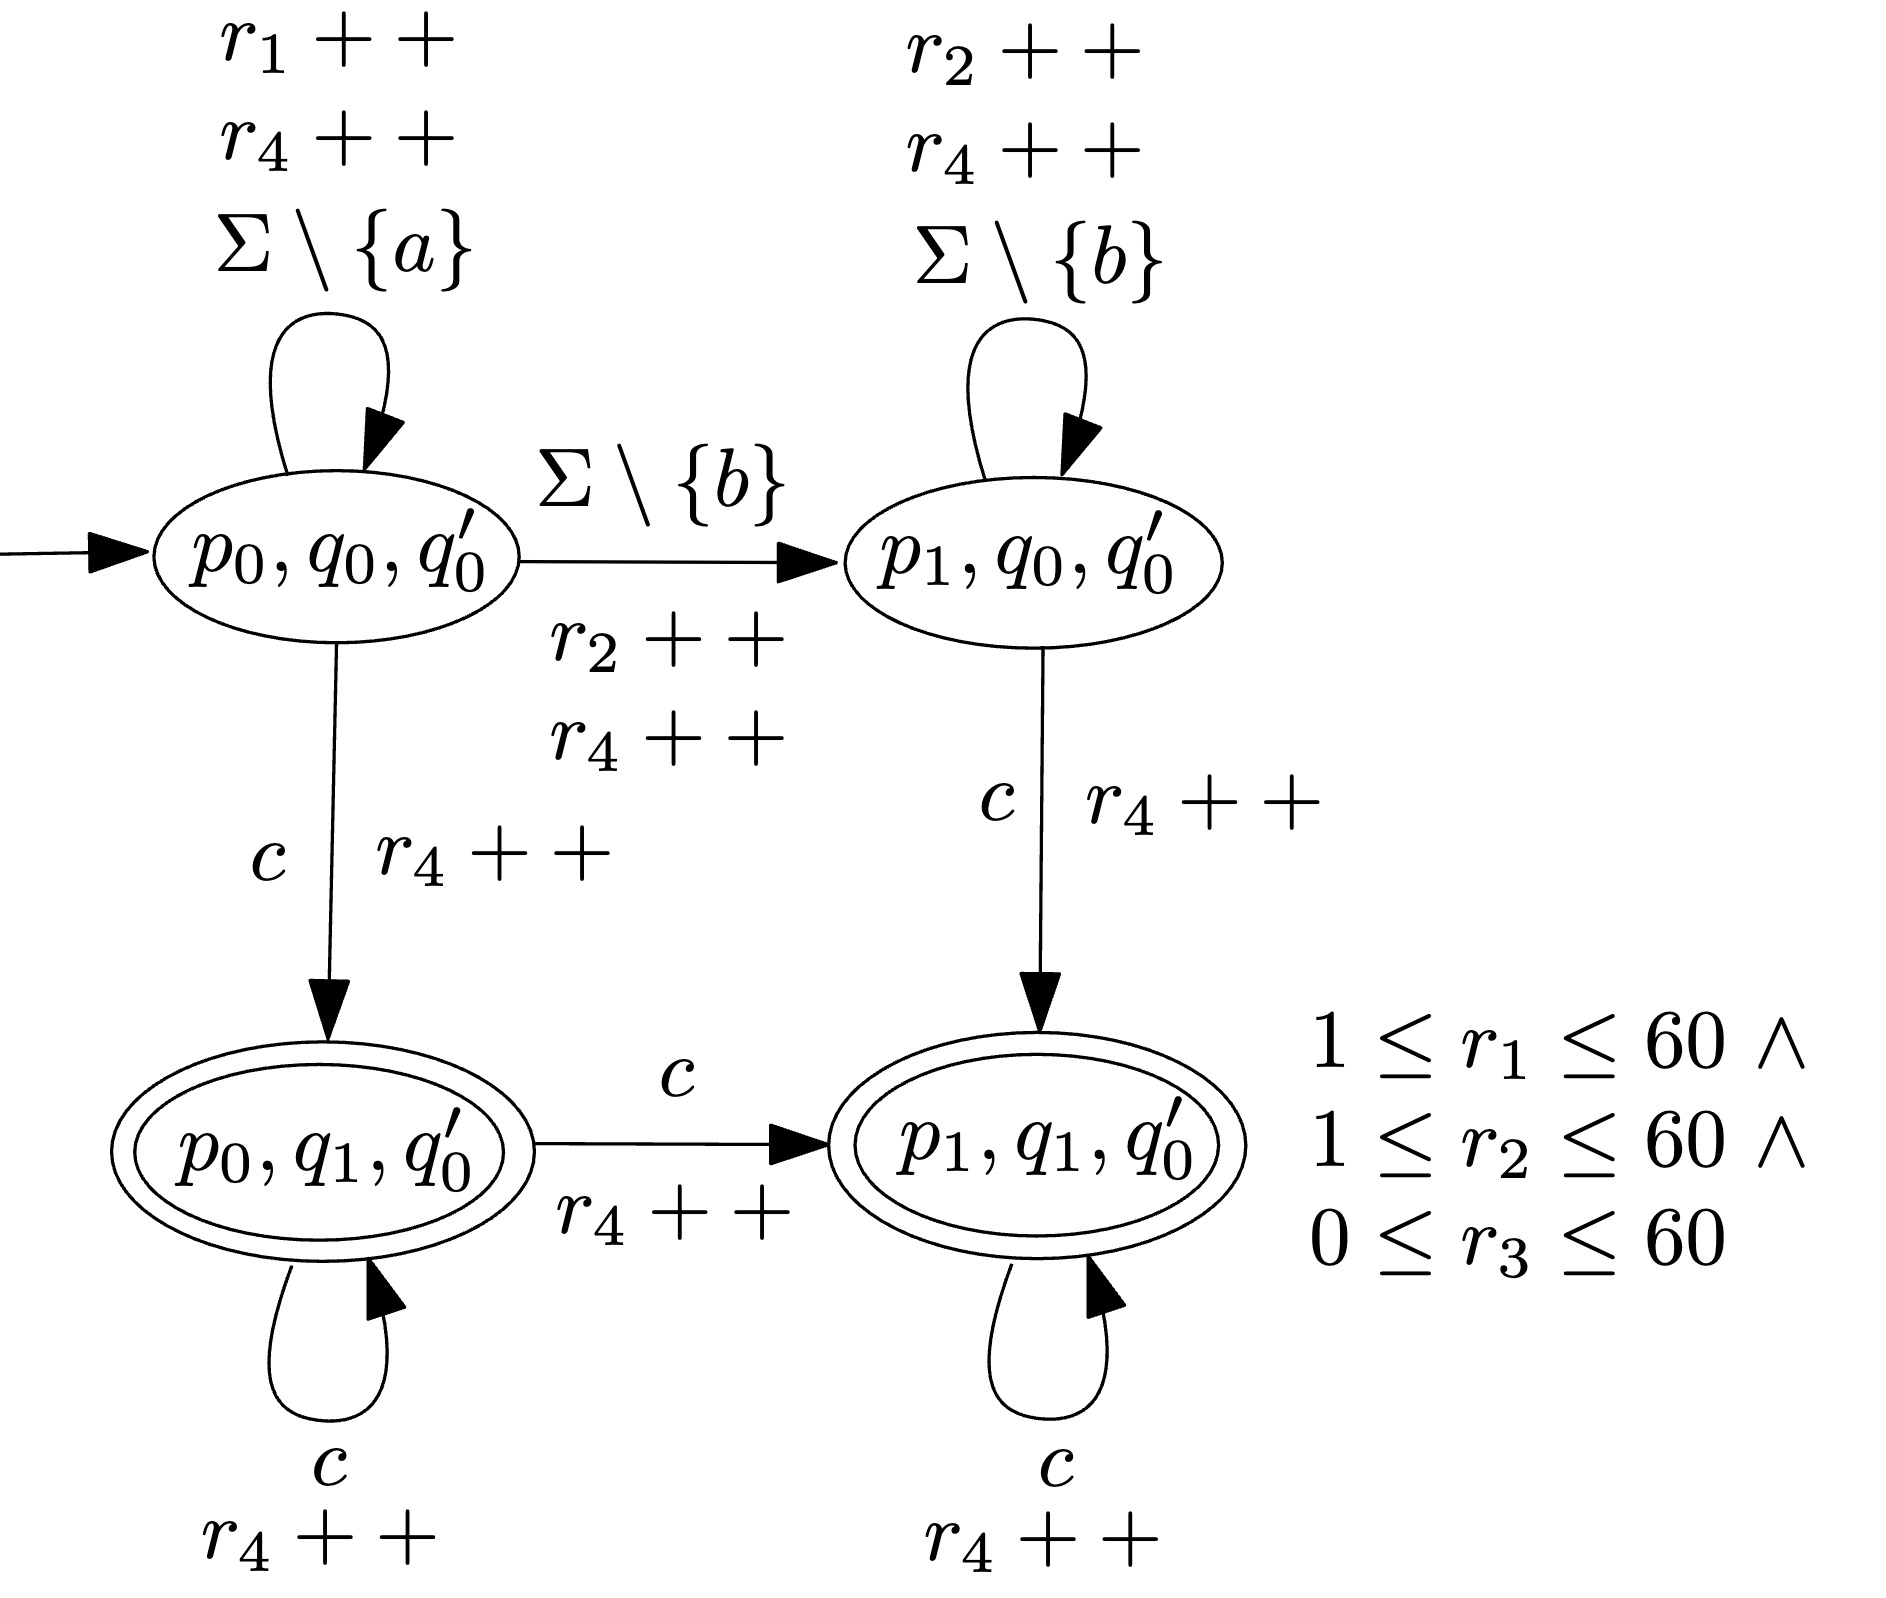
\includegraphics[width=.65\linewidth]{overview_product.jpg}
  \end{figure}
\end{frame}
\begin{frame}{$ x\in (\Sigma / a)^{\{1,60\}}(\Sigma / b)^{\{1,60\}}(\Sigma / c)^{\{0,60\}} \wedge x\in \Sigma^*c^+ \wedge |x| > 120$}
  \textbf{2. Abstract the Updates of Registers as Vectors : }
  \begin{figure}
    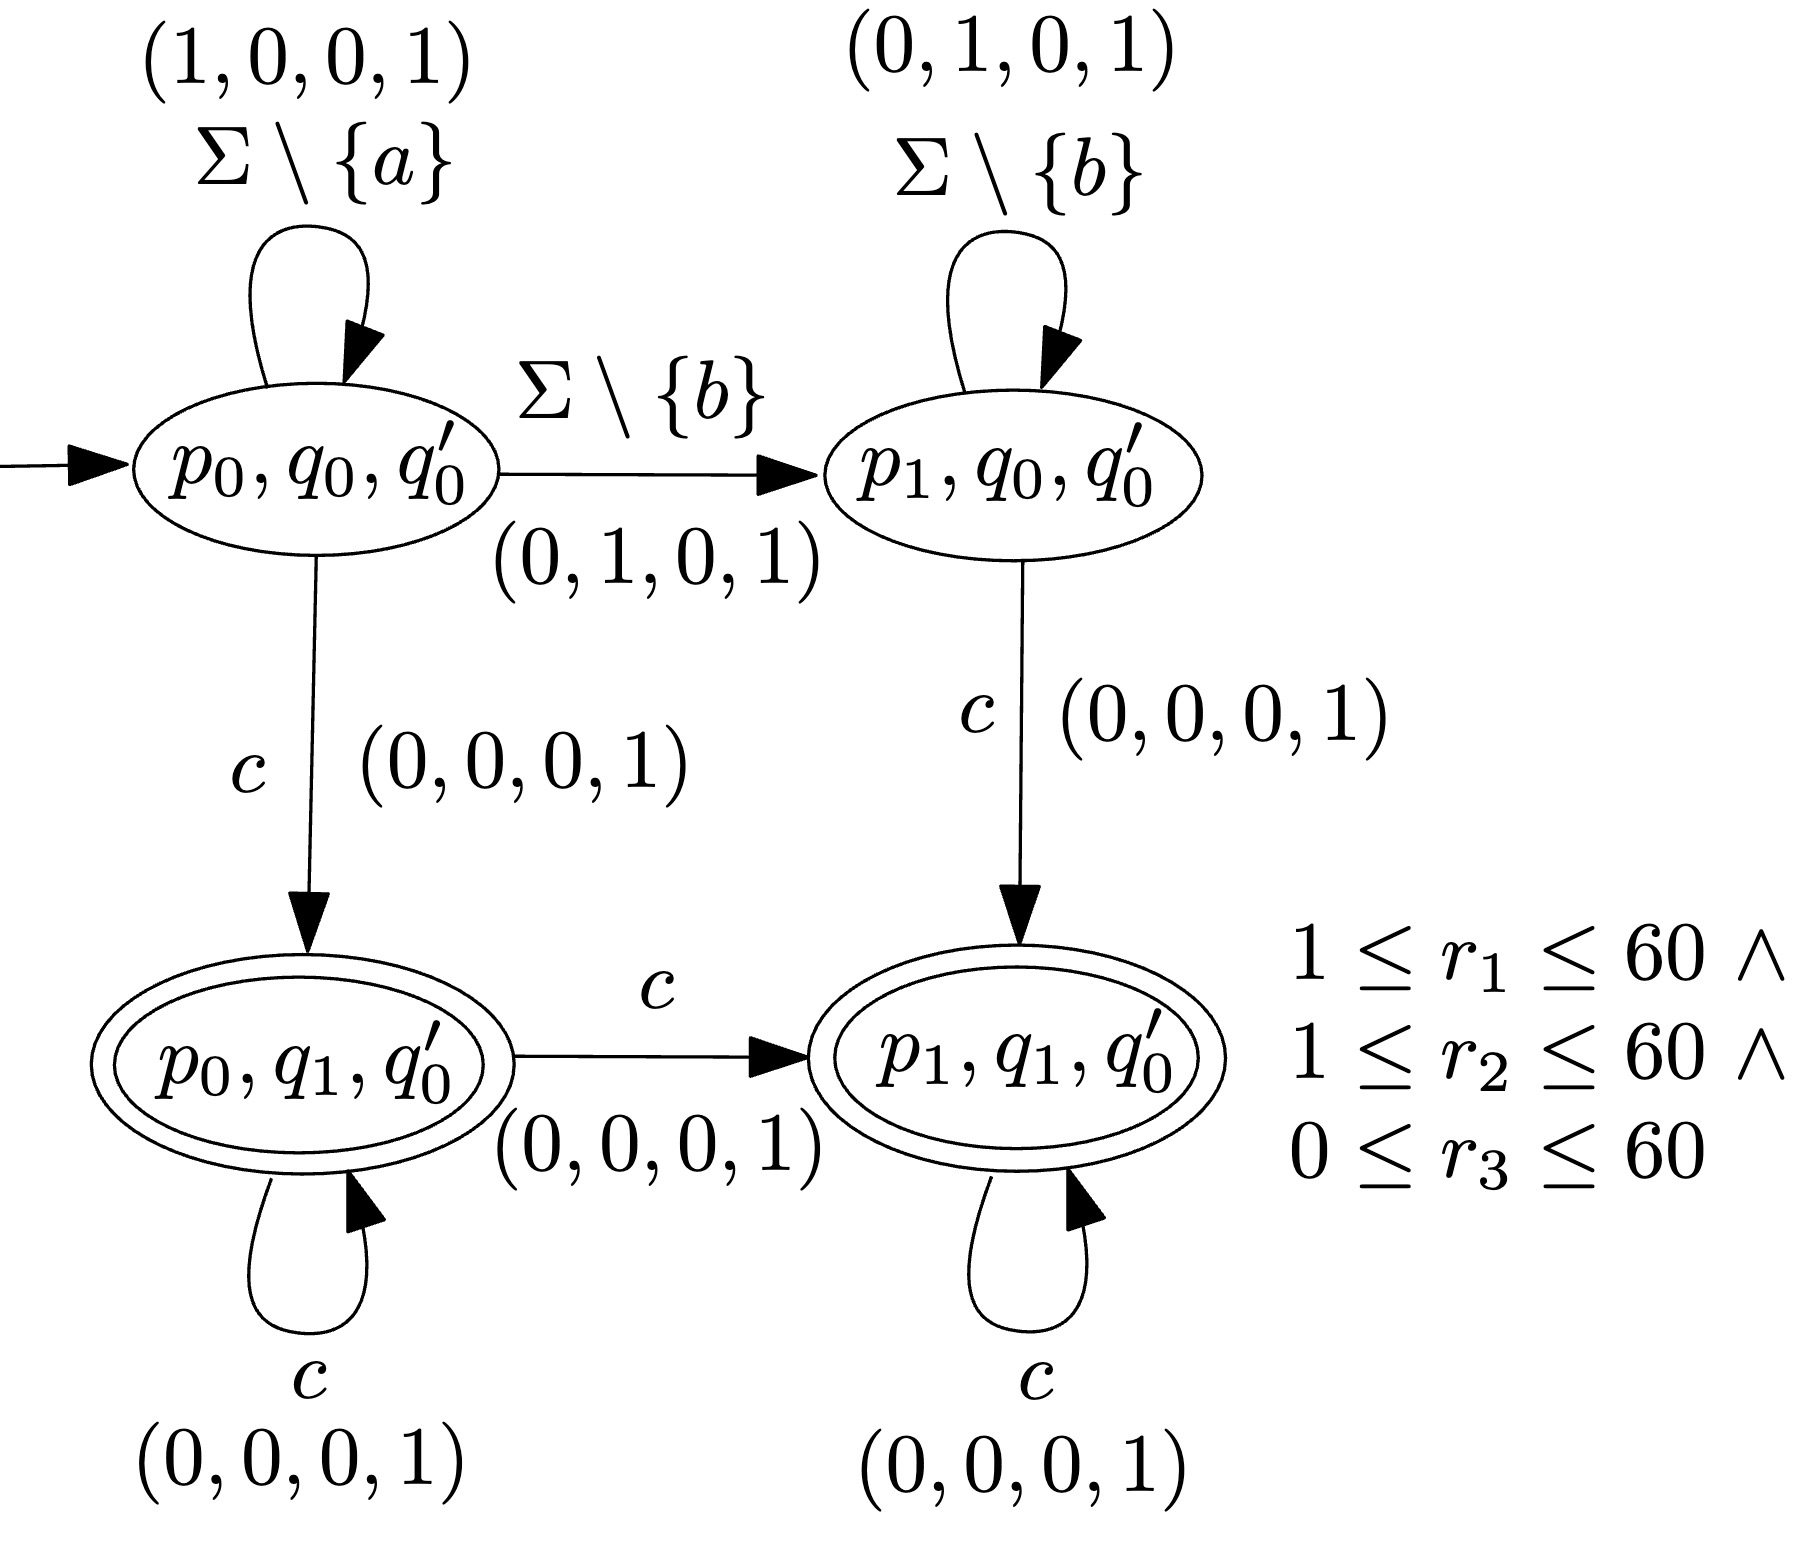
\includegraphics[width=.65\linewidth]{overview_product_vector.jpg}
  \end{figure}
\end{frame}
\begin{frame}{$ x\in (\Sigma / a)^{\{1,60\}}(\Sigma / b)^{\{1,60\}}(\Sigma / c)^{\{0,60\}} \wedge x\in \Sigma^*c^+ \wedge |x| > 120$}
  \textbf{2. Size-Reduction of the Automaton : }
  \begin{figure}
    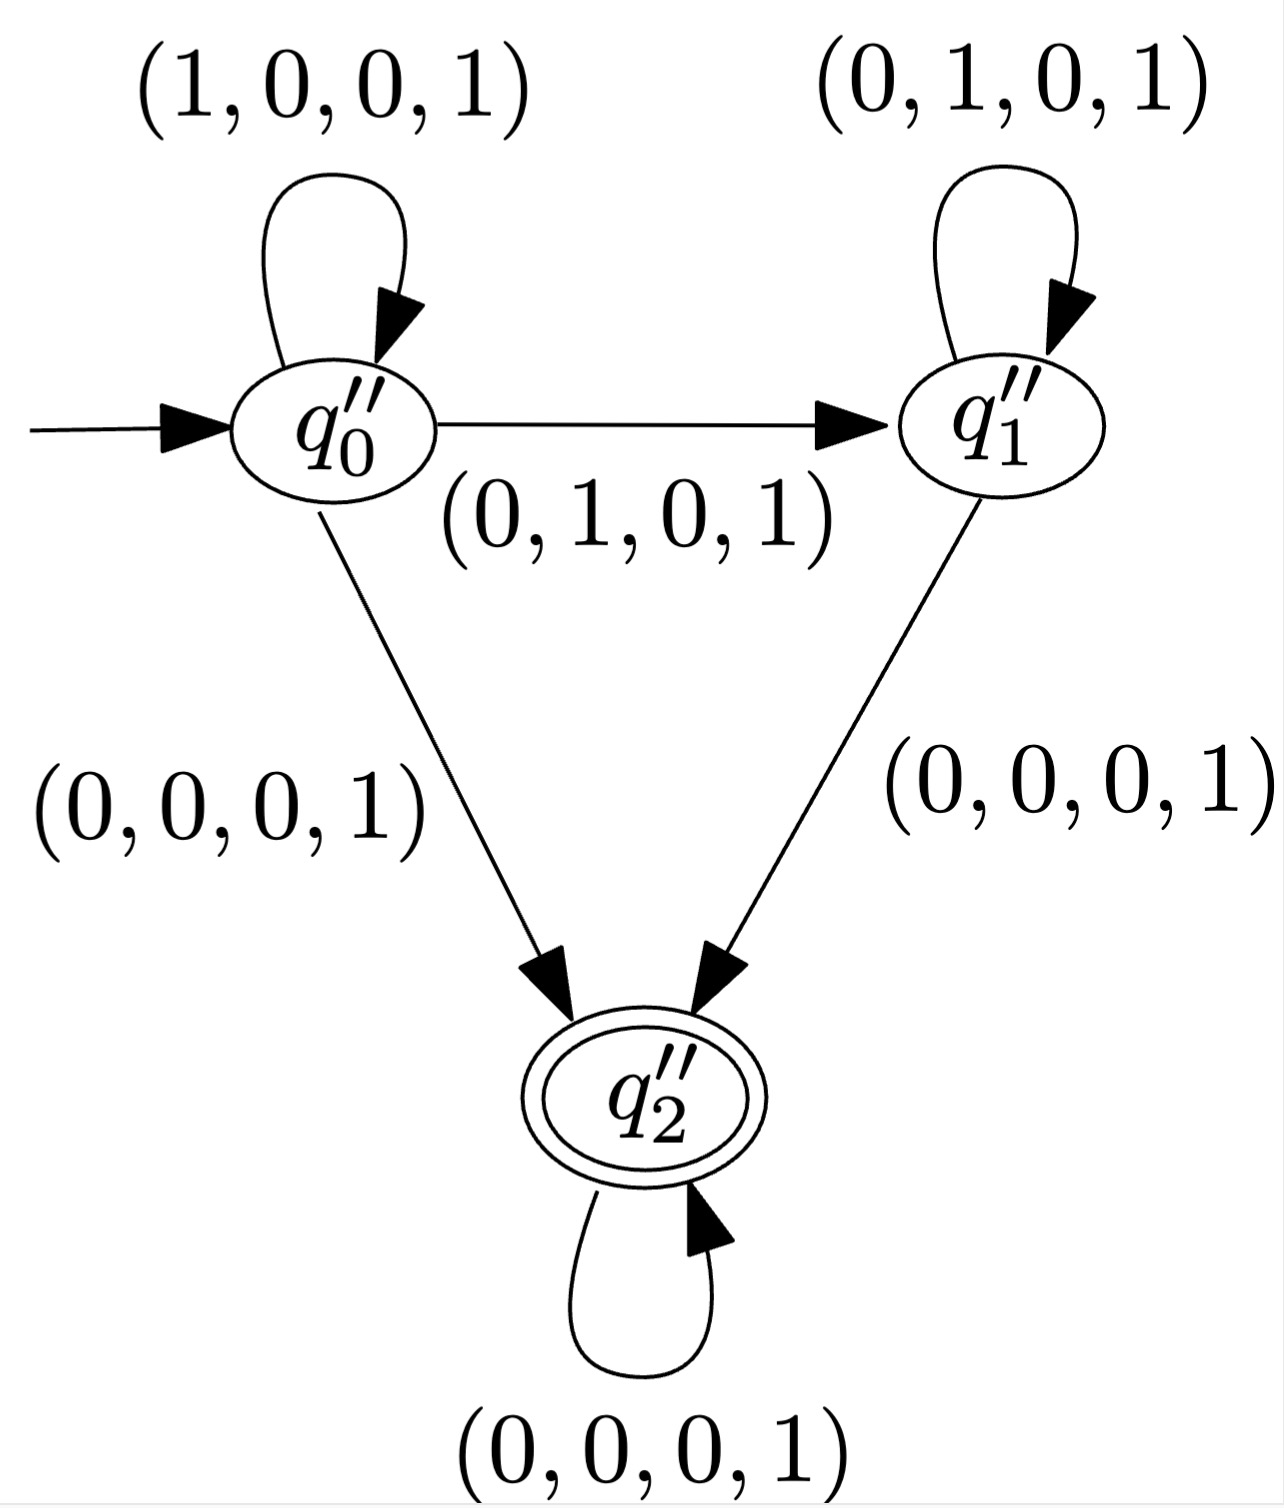
\includegraphics[width=.45\linewidth]{overview_product_vector_simplify.jpg}
  \end{figure}
\end{frame}

\begin{frame}{$ x\in (\Sigma / a)^{\{1,60\}}(\Sigma / b)^{\{1,60\}}(\Sigma / c)^{\{0,60\}} \wedge x\in \Sigma^*c^+ \wedge |x| > 120$}
  \textbf{3. Reduce the Automaton to Parikh Images : }
  \begin{equation}\label{eqn-LIA}
    \begin{array}{l}
      \textcolor{red}{\psi_\cB(\anivar_1, \cdots, \anivar_m)} \wedge \bigwedge \limits_{1 \le j \le 4} r_j = \sum \limits_{1\le k \le m}  \anivar_k v_{k, j}\ \wedge \\
      1 \le r_1 \le 60 \wedge 1 \le r_2 \le 60 \wedge 0 \le r_3 \le 60 \wedge r_4 > 120.
    \end{array}
  \end{equation}
  \begin{tikzpicture}
    \node [opacity = 0] (placeholder) at (0,0) { \textbf{4. Solve the Parikh Images by the SMT Solver (Princess)} };
    \node [rotate=45, scale=1.8, text=green!90!black, fill=yellow!20,draw,decorate,decoration={bumps,mirror}, opacity = 0] at (0,0) {1s SOLVED!!!};
  \end{tikzpicture}
\end{frame}
\begin{frame}{$ x\in (\Sigma / a)^{\{1,60\}}(\Sigma / b)^{\{1,60\}}(\Sigma / c)^{\{0,60\}} \wedge x\in \Sigma^*c^+ \wedge |x| > 120$}
  \textbf{3. Reduce the Automaton to Parikh Images : }
  \begin{equation}\label{eqn-LIA}
    \begin{array}{l}
      \textcolor{red}{\psi_\cB(\anivar_1, \cdots, \anivar_m)} \wedge \bigwedge \limits_{1 \le j \le 4} r_j = \sum \limits_{1\le k \le m}  \anivar_k v_{k, j}\ \wedge \\
      1 \le r_1 \le 60 \wedge 1 \le r_2 \le 60 \wedge 0 \le r_3 \le 60 \wedge r_4 > 120.
    \end{array}
  \end{equation}
  \begin{tikzpicture}
    \node (placeholder) at (0,0) { \textbf{4. Solve the Parikh Images by the SMT Solver (Princess)} };
    \node [rotate=45, scale=1.8, text=green!90!black, fill=yellow!20,draw,decorate,decoration={bumps,mirror}, opacity = 0] at (0,0) {1s SOLVED!!!};
  \end{tikzpicture}
\end{frame}
\begin{frame}{$ x\in (\Sigma / a)^{\{1,60\}}(\Sigma / b)^{\{1,60\}}(\Sigma / c)^{\{0,60\}} \wedge x\in \Sigma^*c^+ \wedge |x| > 120$}
  \textbf{3. Reduce the Automaton to Parikh Images : }
  \begin{equation}\label{eqn-LIA}
    \begin{array}{l}
      \textcolor{red}{\psi_\cB(\anivar_1, \cdots, \anivar_m)} \wedge \bigwedge \limits_{1 \le j \le 4} r_j = \sum \limits_{1\le k \le m}  \anivar_k v_{k, j}\ \wedge \\
      1 \le r_1 \le 60 \wedge 1 \le r_2 \le 60 \wedge 0 \le r_3 \le 60 \wedge r_4 > 120.
    \end{array}
  \end{equation}
  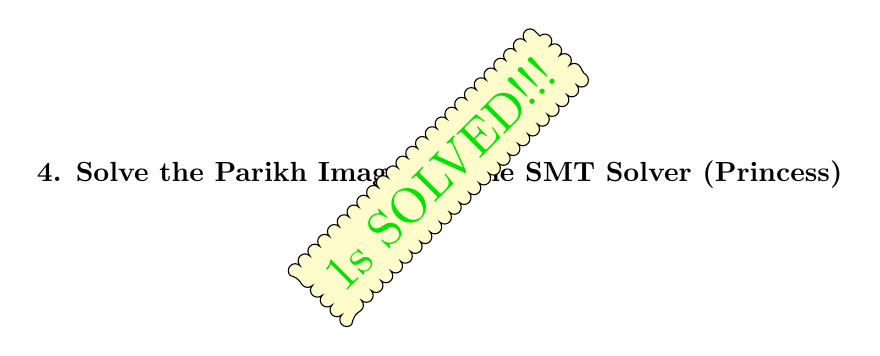
\begin{tikzpicture}
    \node (placeholder) at (0,0) { \textbf{4. Solve the Parikh Images by the SMT Solver (Princess)} };
    \node [rotate=45, scale=1.8, text=green!90!black, fill=yellow!20,draw,decorate,decoration={bumps,mirror}] at (0,0) {1s SOLVED!!!};
  \end{tikzpicture}
\end{frame}

% \begin{frame}{Automaton-based}
%   \begin{definition}[Cost-Enriched Finite Automaton]
%     A cost-enriched finite automaton $\aut$ is a tuple $(R, Q, \Sigma, \delta, I, F, \alpha)$ where
%     \begin{itemize}
%       \item $R = \{r_1, \cdots, r_k\}$ is a finite set of registers,
%       \item $Q, \Sigma, I, F$ are as in the definition of NFA,
%       \item $\delta \subseteq Q \times \Sigma \times Q \times \mathbb{Z}^R$ is a transition relation, where $\mathbb{Z}^R$ denotes the updates on the values of registers.
%       \item $\alpha \in \Phi(R)$ is an LIA formula specifying an accepting condition.
%     \end{itemize}
%   \end{definition}
% \end{frame}

% \begin{frame}{Automaton-based}
%   Let $\aut = (R, Q, \Sigma, \delta, I, F, \alpha)$ be a CEFA.
%   \begin{run}
%     A \emph{run} of $\aut$ on a string $w = a_1 \cdots a_n$ is a sequence $q_0 \xrightarrow[\myvec{v_1}]{a_1} q_1 \cdots q_{n-1}\xrightarrow[\myvec{v_n}]{a_n} q_n$ such that $q_0 \in I$ and $q_{i-1} \xrightarrow[\myvec{v_i}]{a_i} q_i$ for each $i \in [n]$.
%   \end{run}

%   \begin{accepting}
%     A run $q_0 \xrightarrow[\myvec{v_1}]{a_1} q_1 \cdots q_{n-1}\xrightarrow[\myvec{v_n}]{a_n} q_n$ is \emph{accepting} if $q_n \in F$ and $\alpha(\myvec{v'}/R)$ is true, where $\myvec{v'} = \sum \limits_{j \in [n]} \myvec{v_j}$
%   \end{accepting}

% \end{frame}

% \begin{frame}{Symbolically encoding}
%   illustrate the CEFA of regexes in the example. explain why it is symbolic and what the difference is compared to unwinding
% \end{frame}

% \begin{frame}{Size reduction techniques}
%   trival minimization: (a, v) together as one symbol
%   but not enough
% \end{frame}

% \begin{frame}{Size reduction techniques}
%   only consider vectors, i.e., the alphabet is unary. and let 0 vector be epsilon label. do the minimization techniques.

%   significantly improve the preformance. (show the data)
% \end{frame}

\begin{frame}{The Brief of Decision Procedure}
  \begin{enumerate}
    \item Encode counting operators by the automata with registers.
    \item Product the automata and simplify them.
    \item Convert them to parikh images.
    \item Solve the parikh images by the SMT solver (Princess).
  \end{enumerate}
\end{frame}


% Experiment Results (3min)
% 1 Introduction of benchmark suites
% 2 Explanation for results
\section{Evaluation}

\begin{frame}{System Overview}
  \begin{figure}[!htb]
    \centering
    \resizebox{\textwidth}{!}{ % Resize the TikZ picture to fit the frame width
      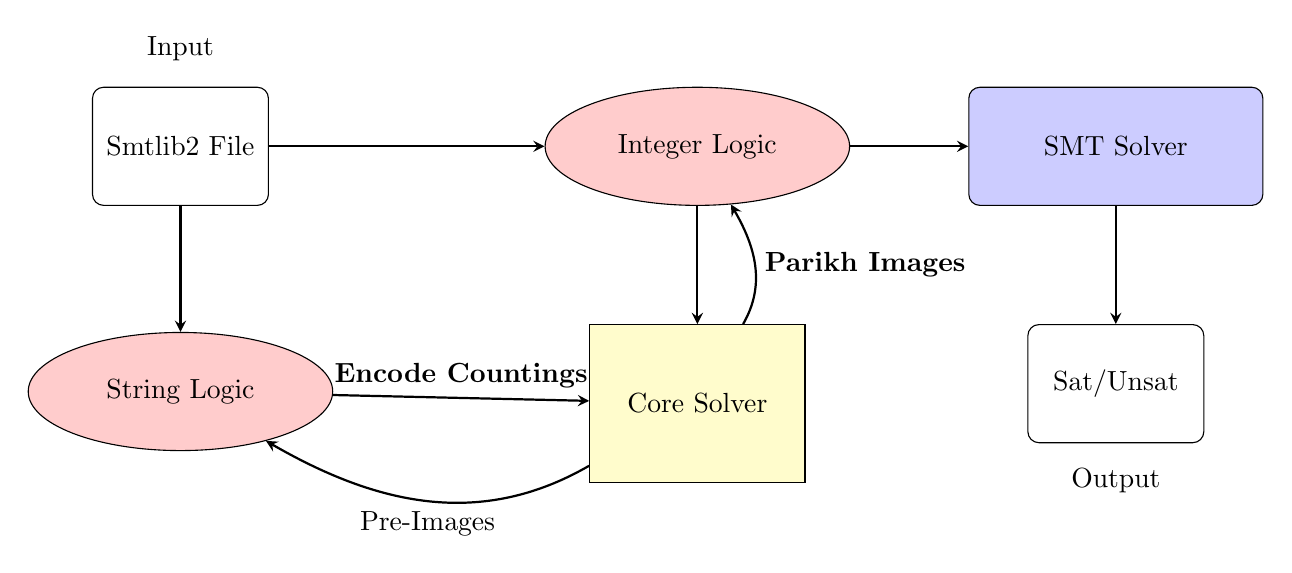
\begin{tikzpicture}[>=latex]

        % Define block styles
        \tikzstyle{input} = [rectangle, draw, fill=white!20, text width=2cm, text centered, rounded corners, minimum height=1.5cm]
        \tikzstyle{output} = [rectangle, draw, fill=white!20, text width=2cm, text centered, rounded corners, minimum height=1.5cm]
        \tikzstyle{component} = [rectangle, draw, fill=blue!20, text width=3.5cm, text centered, rounded corners, minimum height=1.5cm]
        \tikzstyle{core} = [rectangle, draw, fill=yellow!20, text width=2.5cm, text centered, minimum height=2cm]
        \tikzstyle{logic} = [ellipse, draw, fill=red!20, text width=2.5cm, text centered, minimum height=1.5cm]
        \tikzstyle{file} = [rectangle, draw, fill=green!20, text width=1.5cm, text centered, rounded corners, minimum height=1cm]
        \tikzstyle{arrow} = [thick,->,>=stealth]

        % Components
        \node (input) [input] {Smtlib2 File};
        \node (integer) [logic, right=3.5cm of input] {Integer Logic};
        \node (core) [core, below=1.5cm of integer] {Core Solver};
        \node (string) [logic, below=1.6cm of input] {String Logic};
        \node (smtsolver) [component, right=1.5cm of integer] {SMT Solver};
        \node (output) [output, below=1.5cm of smtsolver] {Sat/Unsat};

        % Arrows
        \draw [arrow] (input) -- (integer);
        \draw [arrow] (integer) -- (core);
        \draw [arrow] (core) to[out=60,in=-60] node[midway, right] {\textbf{Parikh Images}} (integer);
        \draw [arrow] (input) -- (string);
        \draw [arrow] (string) to node[midway, above] {\textbf{Encode Countings}} (core);
        \draw [arrow] (core) to[out=-150,in=-30] node[midway, below] {Pre-Images} (string);
        \draw [arrow] (integer) -- (smtsolver);
        \draw [arrow] (smtsolver) -- (output);

        % Labels
        \node [above=0.2cm of input] {Input};
        \node [below=0.2cm of output] {Output};

      \end{tikzpicture}
    }
  \end{figure}

\end{frame}

\begin{frame}{Benchmark Suites and Environment}
  \begin{benchmark}
    \begin{itemize}
      \item \textbf{RegCoL:} 40,628 instances that contains regexes from real-world website and is manually constructed.
      \item \textbf{AutomatArk:}  8,215 instances that is adapted from the AutomatArk suite.
    \end{itemize}
  \end{benchmark}
\end{frame}

\begin{frame}{Benchmark Suites and Environment}
  \begin{distribution}
    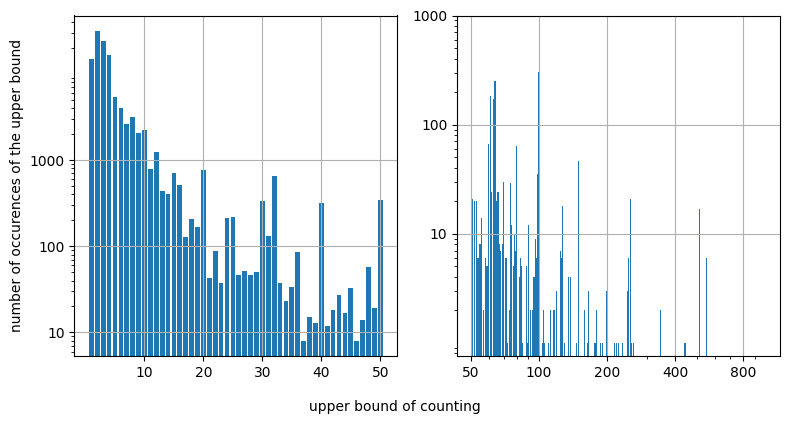
\includegraphics[width=\linewidth]{counting_distribution.png}
  \end{distribution}
\end{frame}

\begin{frame}{Benchmark Suites and Environment}
  \begin{environment}
    \begin{itemize}
      \item \textbf{Operating System: } CentOS Stream release 8
      \item \textbf{CPU: } Intel(R) Xeon(R) Platinum 8269CY 3.10GHz
      \item \textbf{Memory: } 190 GB
      \item \textbf{Timeout Limit: } 60s
    \end{itemize}
  \end{environment}
\end{frame}

\begin{frame}{Our Solver Solve the Most Instances}
  \centering
  \usepgfplotslibrary{fillbetween}
\pgfplotsset{compat=1.16}
\resizebox{.95\textwidth}{!}{\begin{tabular}{|>{\centering\arraybackslash}m{1.45cm} |c |c |c |c |c |c |}
            \hline
                                                     & CVC5       & Z3str3RE      & Z3str3 & Z3seq & \textsc{Ostrich} & $\ostrichrecl$ \\
            \hline
            \hline

            \rowcolor{grayshade} sat                 & 27813      & 28283         & 23126  & 27761 & 25975            & \textbf{28360} \\
            \hline
            \rowcolor{grayshade} unsat               & 16941      & 19312         & 12742  & 18651 & 20291            & \textbf{20302} \\
            \hline
            \hline

            unknown                                  & \textbf{8} & 99           & 6990   & 98    & 160              & 28             \\
            \hline
            timeout                                  & 4081       & 1149          & 5985   & 2333  & 2417             & \textbf{153}   \\
            \hline
            soundness  error                         & \textbf{0} & 44            & 44     & 56    & \textbf{0}       & \textbf{0}     \\
            \hline
            \hline
            \rowcolor{grayshade} solved\quad  correctly & 44754      & 47551         & 35824  & 46356 & 46266            & \textbf{48662} \\
            \hline
            \rowcolor{grayshade} average  time (s)   & 5.64       & \textbf{1.62} & 7.63   & 3.59  & 5.94             & 1.93           \\
            \hline
      \end{tabular}}
\end{frame}

\begin{frame}{Our Technical Choises Are the Most Efficient}
  \centering
  \usepgfplotslibrary{fillbetween}
\pgfplotsset{compat=1.16}
\resizebox{.95\textwidth}{!}{\begin{tabular}{|>{\centering\arraybackslash}m{1.45cm} |c |c |c |}
    \hline
                                           & $\ostrichrecl_{\rm -ASR}$  & $\ostrichrecl_{\rm NUXMV}$  & $\ostrichrecl$ \\
    \hline\hline
    \rowcolor{grayshade} sat               & \mycomment{26884+411}27295 & \mycomment{26603 +4}26607   & \textbf{29084} \\
    \hline
    \rowcolor{grayshade} unsat             & \mycomment{20275+238}20513 & \mycomment{20261 +238}20499 & \textbf{20554} \\
    \hline
    \hline
    unknown                                & \mycomment{48+20}68        & \mycomment{45+0}45          & \textbf{14}    \\
    \hline
    timeout                                & \mycomment{1637+331}1968   & \mycomment{1935 +758}2693   & \textbf{191}   \\
    \hline
    error                                  & \textbf{0}                 & \textbf{0}                  & \textbf{0}     \\
    \hline
    \hline
    \rowcolor{grayshade} solved            & \mycomment{47159+649}47808 & \mycomment{46864 +242}47106 & \textbf{49638} \\
    \hline
    \rowcolor{grayshade} average  time (s) & \mycomment{4.27+28.91}4.76 & \mycomment{6.05 +46.31}6.86 & \textbf{2.88}  \\
    \hline
  \end{tabular}}
\end{frame}

% Summary and Future work (1min)
% 1 contribution again and main points
% 2 how to handle non-register-representable counting
% 3 potential application 
\section{Conclusion and Future Work}
\begin{frame}
  \frametitle{Our Contributions}
  \begin{enumerate}
    \item Divise an algorithm that efficiently solve string constraints with regex-counting and string-length
    \item Propose particular size-reduction techniques for automata with registers
    \item Carry out abundant experiments
  \end{enumerate}
\end{frame}


\begin{frame}
  \frametitle{Future Work}
  \begin{enumerate}
    \item Symbolically encode non-register-representable counting operators, such as $(a^{\{1,3\}})^*$ and $\overline{a^{\{1,3\}}}$.
    \item Apply this method in the analysis of real-world programs.
  \end{enumerate}
\end{frame}

\end{document}